%% rnaastex.cls is the classfile used for Research Notes. It is derived
%% from aastex61.cls with a few tweaks to allow for the unique format required.
%% (10/15/17)
%%\documentclass{rnaastex}

%% Better is to use the "RNAAS" style option in AASTeX v6.2
%% (01/08/18)
\documentclass[RNAAS]{aastex631}

%% Define new commands here
\newcommand\latex{La\TeX}

\begin{document}

\title{NGC 1605 is not a binary cluster}

%% Note that the corresponding author command and emails has to come
%% before everything else. Also place all the emails in the \email
%% command instead of using multiple \email calls.
%\correspondingauthor{Friedrich Anders}
%\email{fanders@fqa.ub.edu}

%% The \author command can take an optional ORCID.
\author[0000-0003-4524-9363]{Friedrich Anders}
\affiliation{Institut de Ci\`encies del Cosmos, Universitat de Barcelona (IEEC-UB), Mart\'i i Franqu\`es 1, 08028 Barcelona, Spain}

\author[0000-0002-9419-3725]{Alfred Castro-Ginard}
\affiliation{Leiden Observatory, Leiden University, Niels Bohrweg, 2, 2333CA Leiden, The Netherlands}

\author[0000-0003-4105-2520]{Juan Casado}
\affiliation{Facultat de Ciències, Universitat Autònoma de Barcelona (UAB), 08193 Bellaterra, Barcelona, Spain}

\author[0000-0001-5495-9602]{Carme Jordi}
\affiliation{Institut de Ci\`encies del Cosmos, Universitat de Barcelona (IEEC-UB), Mart\'i i Franqu\`es 1, 08028 Barcelona, Spain}

%% Note that RNAAS manuscripts DO NOT have abstracts.
%% See the online documentation for the full list of available subject
%% keywords and the rules for their use.
\keywords{open clusters --- NGC 1605 --- Gaia EDR3 --- data analysis}

%% Start the main body of the article. If no sections in the 
%% research note leave the \section call blank to make the title.
\section{Abstract}
The open star cluster NGC 1605 has recently been reported to in fact consist of two clusters (one intermediate-aged and one old) that merged via a flyby capture. Here we show that {\it Gaia} data does not support this scenario. We do, however, find another open-cluster candidate nearby.

\section{Introduction}
Gravitational captures of star clusters by other clusters are very rare and elusive events that can serve as laboratories for the destruction of star clusters (e.g. \citealt{Soubiran2018, Casado2022}). Recently, \citet{Piatti2022} presented a promising candidate for an open cluster collision of the nearby ($d\sim330$ pc) objects IC 4665 and Collinder 350.
Some months earlier, \citet{Camargo2021} reported the existence of a possible binary cluster, dubbed NGC 1605a/b, and suggested that it origined from a flyby capture. The author argued that the long-known cluster NGC 1605 actually consists of two components that have vastly different ages (2 Gyr and 600 Myr). Here we report that {\bf both manual analysis (by each of the authors individually) and} commonly used clustering analysis techniques show no hint for multiple populations in this cluster.

Although relatively distant, close to the Galactic plane, and little studied, NGC 1605 has been included in the Galactic open cluster census since the 1970s. In the first deep photometric analysis, \citet{Fang1970} remarks that "the cluster does not show much concentration but it is detached clearly from the background of a small stellar density which is probably caused by large interstellar absorption". % \citep{Becker1971, Janes1982, Leisawitz1989}. %The precision astrometry of the second data release of {\it Gaia} data \citep{Gaia2016, Gaia2018} has allowed the community to study open clusters in much more detail. 
The object is also listed in the {\it Gaia} DR2 open cluster catalogue of \citet{Cantat2020}, with 95 bona-fide members, an age of 190 Myr, a distance of 3.07 kpc, and a foreground extinction of 2.21 mag.

\section{Gaia EDR3 analysis}
We reanalyse the {\it Gaia} EDR3 data \citep{Gaia2021} down to magnitude $G<19$ in a 30 arcmin circle around the centre of NGC 1605. {\bf After a manual analysis leading to the same results, we carry out a blind} analysis\footnote{reproducible at \url{https://github.com/fjaellet/ngc1605}} using the three state-of-the-art clustering techniques that have been introduced in the field: The DBSCAN algorithm employed by \citet{Castro2022}, the pyUPMASK code \citep{Pera2021}, and HDBSCAN, the preferred method of \citet{Hunt2021}. 
While the former algorithms yield only one cluster in the considered region (NGC 1605), HDBSCAN does find another candidate close by - located about 20 arcmin northwest of NGC 1605 and clearly visible as an overdensity in proper-motion space (see Fig. \ref{fig:1}).

NGC 1605's stellar density on the sky looks slightly irregular at first sight (it seems to be missing stars in its centre). It is, however, at all radii 2$\sigma$-consistent with a typical King profile. There are also no irregularities in proper motion or in parallax space. We find no evidence for the tidal streams claimed by \citet{Camargo2021} - their claimed location would also be dynamically inconsistent with the proper motion of the putative sub-clusters.
The second sequence that \citet{Camargo2021} found in the infra-red colour-magnitude diagram of the region (their Fig. 6) is produced by poorly removed field-star contamination (see Sect. 4 of \citealt{CantatAnders2020} for a discussion).
%After testing several sophisticated membership analyses, we use the automated cluster analysis tool ASteCA \citep{Perren2015, Perren2020} to redetermine the astrophysical parameters based on the available astrometric and photometric data. Memberships are obtained with a Bayesian decontamination algorithm computing the likelihood for being a field or a cluster star based on positions, proper motion, and parallax mesurements. The cluster parameters are then determined with a Bayesian isochrone fit to a family of synthetic PARSEC populations including binaries.
%The results of the ASteCA analysis, including the best-fit cluster parameters, are shown in Fig. \ref{fig:1}. The parameters are consistent with the DR2 analysis of \citet{Cantat2020} (which used a neural network trained on well-studied clusters), but thanks to the better precision of {\it Gaia} EDR3 the number of bona-fide members has doubled and the results are slightly more precise. In addition to distance ($d=2600\pm$ pc, age, and extinction ($E(B_V)=1.06\pm0.07$), ASteCA also delivers a photometric metallicity ([Fe/H]$=-0.1\pm0.2$), an , a lower limit for the present-day cluster mass ($\sim 2000 M_{\odot}$), and a binary fraction (in the mass range probed by {\it Gaia} EDR3; $M \gtrsim 1.1M_{\odot}$) of $61\pm16\%$. 

\begin{figure}
\begin{center}
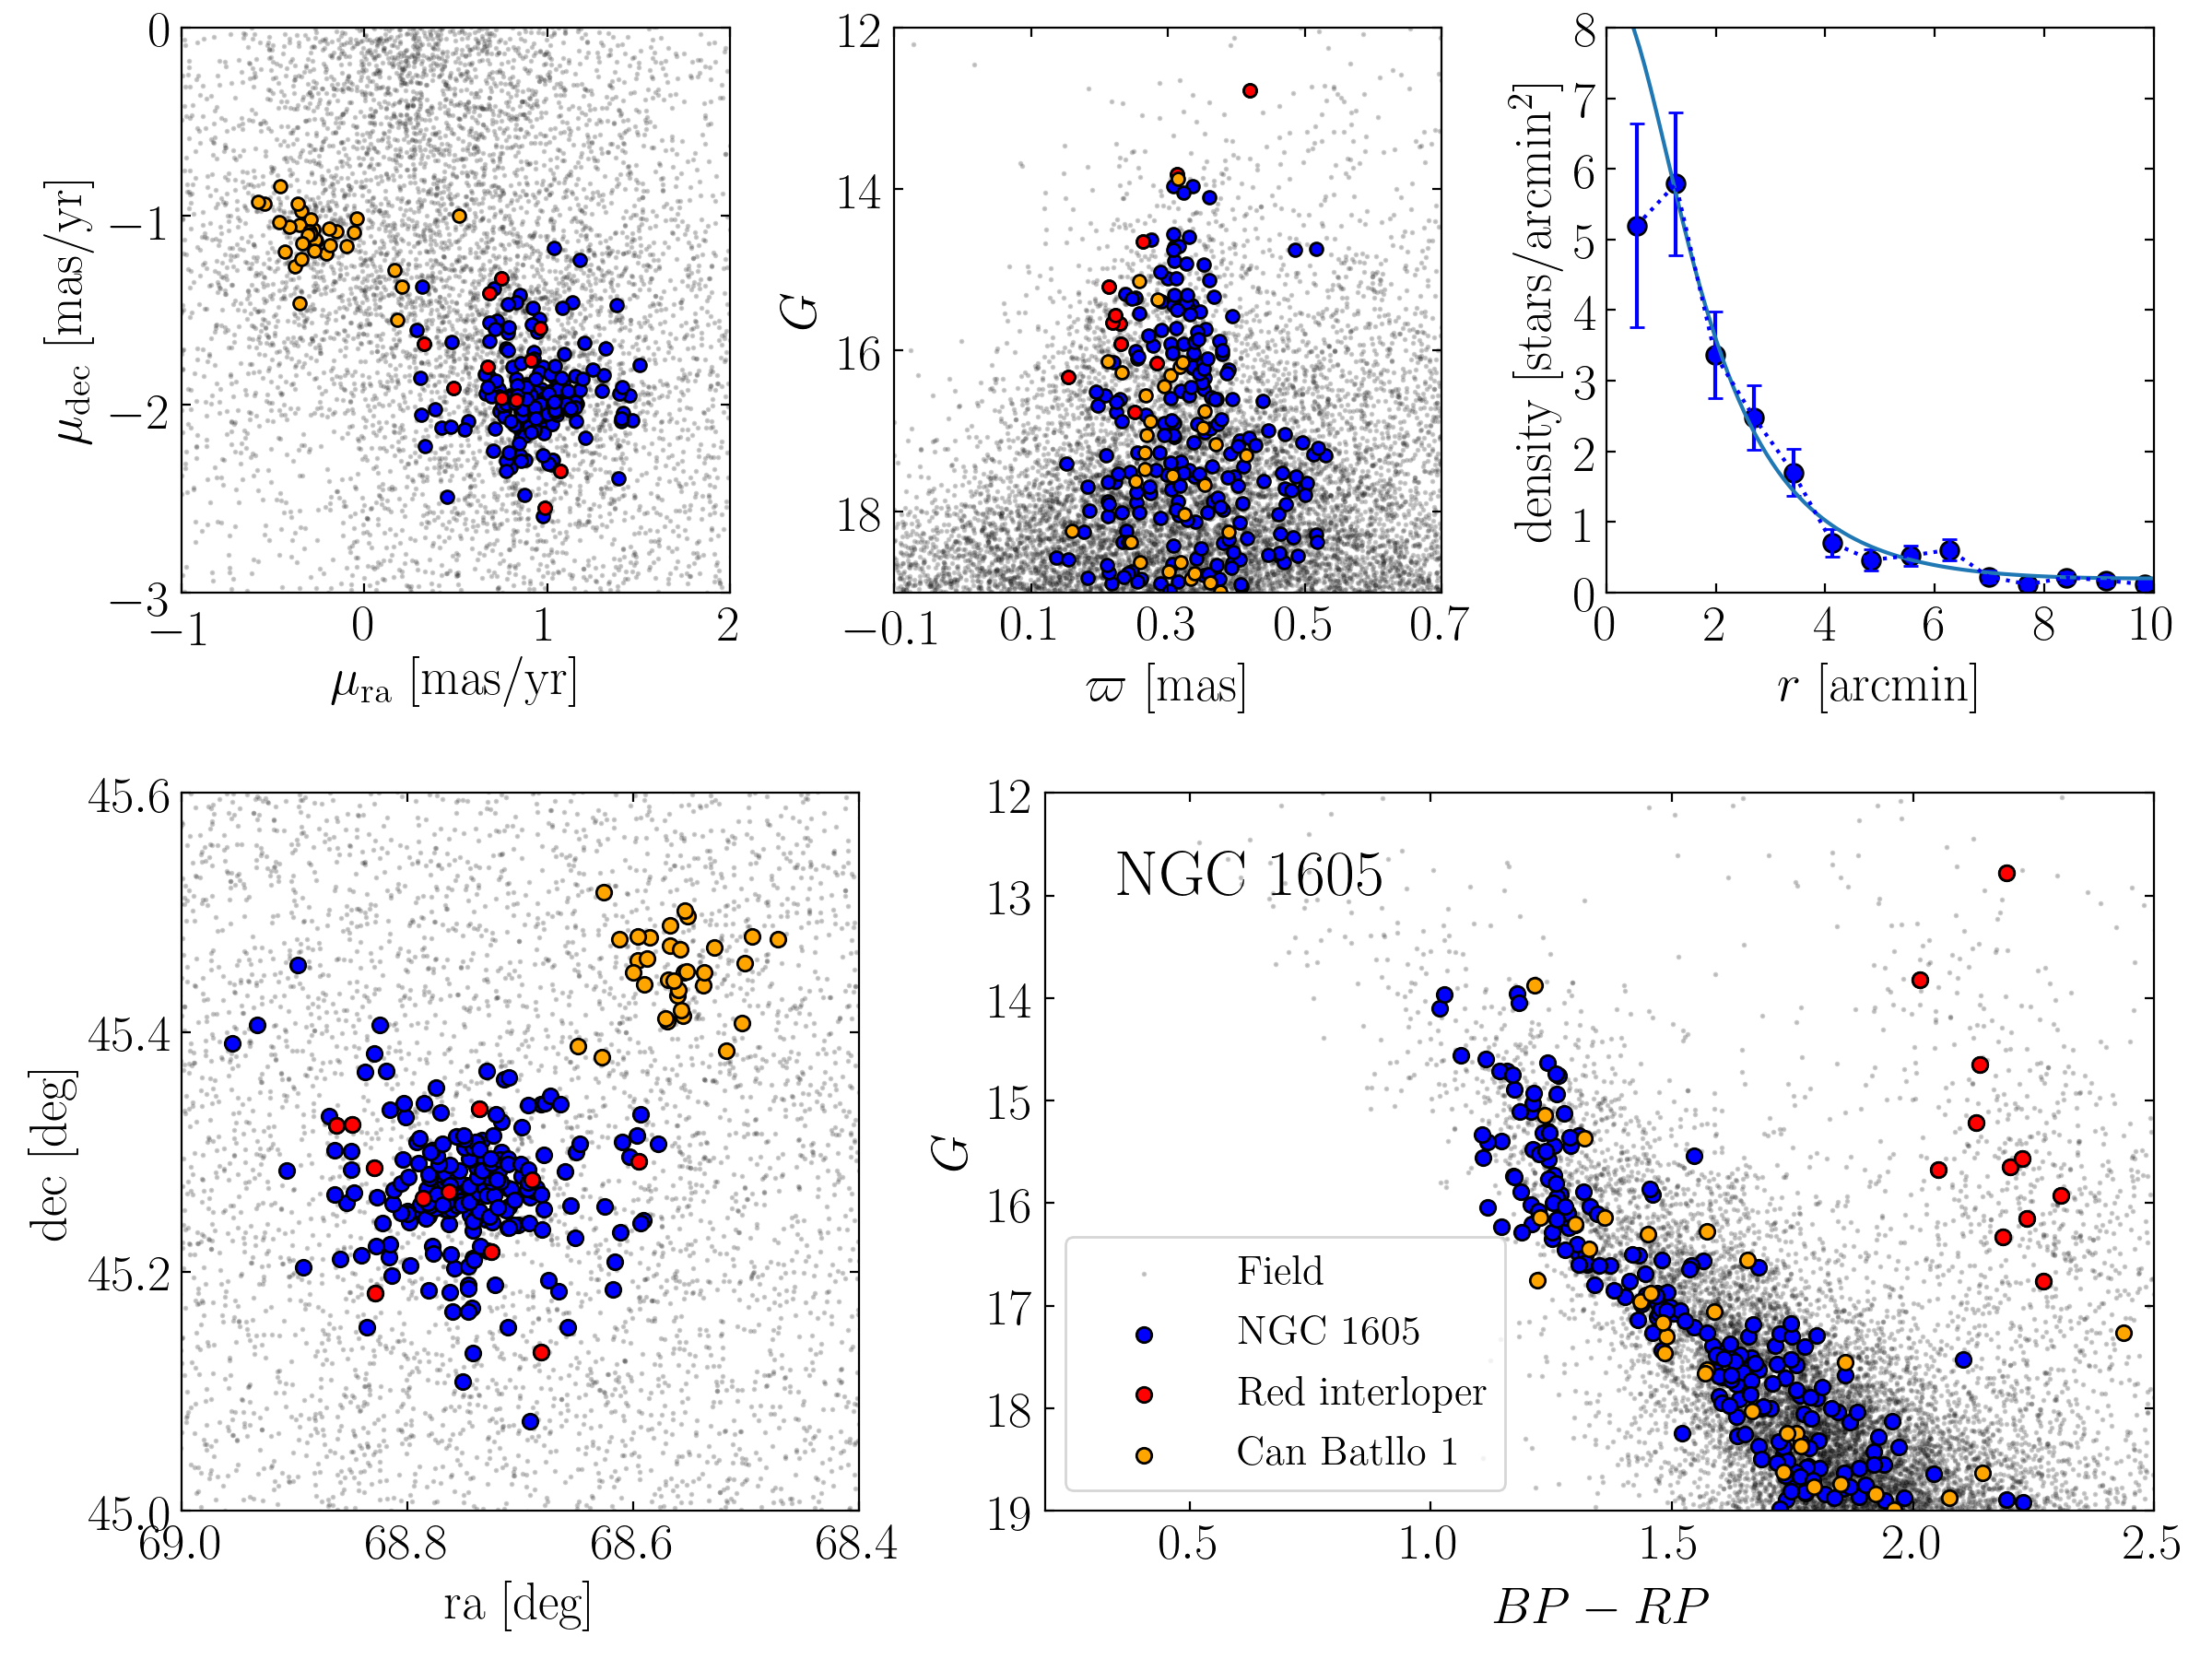
\includegraphics[width=0.88\textwidth,angle=0]{im/ngc1605_hdbscan_analysis.png}
%\caption{AsteCA \citep{Perren2015} analysis of the putative binary cluster NGC 1605. Top left panel: Sky distribution of {\it Gaia} EDR3 stars ($G<19$) in the region of NGC 1605. Top right panel: King profile fit of the stellar density distribution (not taking into account membership analysis yet). The outlying point at 1.75 arcsec is $<2\sigma$-consistent with the best-fit King profile. Bottom row: Results of the MCMC isochrone fit to the colour-magnitude diagram of the NGC 1605 members found in the astrometric analysis. Left: Field-cleaned CMD. Right: Best-fit synthetic PARSEC population. Centre: Hess diagram of the residuals (observed minus synthetic). \label{fig:1}}
\caption{Results of the HDBSCAN analysis of the putative binary cluster NGC 1605. In each panel, the cluster members are highlighted in blue. Other symbols are explained in the legend. Bottom left panel: Sky distribution of {\it Gaia} EDR3 stars ($G<19$) in the region of NGC 1605. Upper left panel: Proper motion diagram. Top middle: Parallax versus magnitude. Top right: density profile (including a King profile with $r_c=2$ arcmin, $r_t=10$ arcmin for comparison). Bottom right panel: Colour-magnitude diagram. Also shown is a {\bf 300 Myr} PARSEC isochrone, shifted by $A_V=2.13$ mag and $(m-M)_0=12.4$ mag. \label{fig:1}}
\end{center}
\end{figure}

In summary, we find no evidence for NGC 1605 being a genuine binary cluster. Nevertheless, NGC 1605 is an intriguing object: Its large Galactocentric distance ($\sim 11$ kpc) makes it an interesting target for spectroscopic follow-up observations. 

%\begin{acknowledgments}
%\end{acknowledgments}

\bibliography{ngc1605}{}
\bibliographystyle{aasjournal}

\end{document}
